\documentclass[10pt]{article}
\usepackage[T1]{fontenc}
\usepackage{lmodern}
\usepackage{amsmath,amssymb,booktabs,graphicx,microtype}
\usepackage[margin=1.75cm]{geometry}
\usepackage{xcolor}
\usepackage[hidelinks]{hyperref}
\definecolor{deepblue}{HTML}{4C78A8}
\definecolor{deeporange}{HTML}{F58518}
\newcommand{\risk}{\mathcal R}
\newcommand{\mse}{\operatorname{MSE}}

\title{Why the Current Reconstruction Error Plateaus\\
\large A diagnostic note on fixed-kernel looped attention}
\author{}
\date{August 4, 2026}

\begin{document}
\maketitle
\vspace{-2.2em}

\begin{abstract}
The present proof of concept does show that prescribing the nonlinear
softmax/RBF feature geometry is useful: the matched loop outperforms both a
standard Transformer and the same loop with a mismatched kernel.  It does
\emph{not}, however, yet produce uniformly accurate reconstructions.  The
reason is primarily informational rather than an optimization failure.  With
12 random measurements, the trained loop has MSE $0.12055$, while the exact
Gaussian-process posterior mean---using the true kernel and noise level---is
already limited to $0.11359$.  Thus $94.2\%$ of the observed error remains
even after replacing the learned iteration by an exact solve.  At budget 8,
the corresponding fraction is $98.0\%$.  A second issue is objective
misalignment: experimental design was trained with a spatial weight that is
$5.78$ times larger at the centre than at the boundary, so a low weighted loss
can coexist with visibly poor boundary reconstruction.  Analytic posterior-risk
calculations show that roughly 16 well-placed measurements, rather than 8, are
needed to cross MSE $10^{-2}$ in this one-dimensional problem.  More training
alone cannot remove this floor.
\end{abstract}

\section{Exact decomposition of the prediction error}

Let $f\sim\mathcal N(0,K)$ on the fixed grid and
$y_C=f_C+\varepsilon$, with
$\varepsilon\sim\mathcal N(0,\sigma^2 I)$.  For a spatial loss matrix
$W=\operatorname{diag}(w)$, the exact posterior mean and covariance are
\begin{align}
 m_C &= K_{:C}(K_{CC}+\sigma^2I)^{-1}y_C,\\
 \Sigma_C &= K-K_{:C}(K_{CC}+\sigma^2I)^{-1}K_{C:}.
\end{align}
For any predictor $\widehat f(y_C)$, posterior orthogonality gives
\begin{equation}
 \underbrace{\mathbb E\|\widehat f-f\|_W^2}_{\text{total risk}}
 =
 \underbrace{\mathbb E_C\operatorname{tr}(W\Sigma_C)}_{\text{information and noise floor}}
 +
 \underbrace{\mathbb E\|\widehat f-m_C\|_W^2}_{\text{solver/model excess}}.
 \label{eq:decomposition}
\end{equation}
Because the data generator uses the same RBF kernel, $\ell=0.18$, and
$\sigma=0.1$, exact KRR with ridge $\lambda=\sigma^2=0.01$ is the Bayes
posterior mean.  It is therefore the correct diagnostic floor for this
protocol, not merely another baseline.

\begin{table}[h]
\centering
\caption{Empirical risk decomposition over five independent training seeds.}
\begin{tabular}{lcccc}
\toprule
Protocol & loop risk & exact GP risk & loop excess & floor/total \\
\midrule
12 random sensors, uniform loss
  & $0.12055$ & $0.11359$ & $0.00696$ & $94.2\%$ \\
8 learned sensors, weighted loss
  & $0.06049$ & $0.05929$ & $0.00120$ & $98.0\%$ \\
\bottomrule
\end{tabular}
\end{table}

The loop is therefore not the dominant bottleneck.  Increasing the tied depth
from 12 to 24 reduces the random-context MSE from approximately $0.1201$ to
$0.1146$, already close to the exact value $0.1136$.  Additional optimizer
steps can at most affect the small second term of
Eq.~\eqref{eq:decomposition}; they cannot reduce posterior uncertainty.

\begin{figure}[p]
\centering
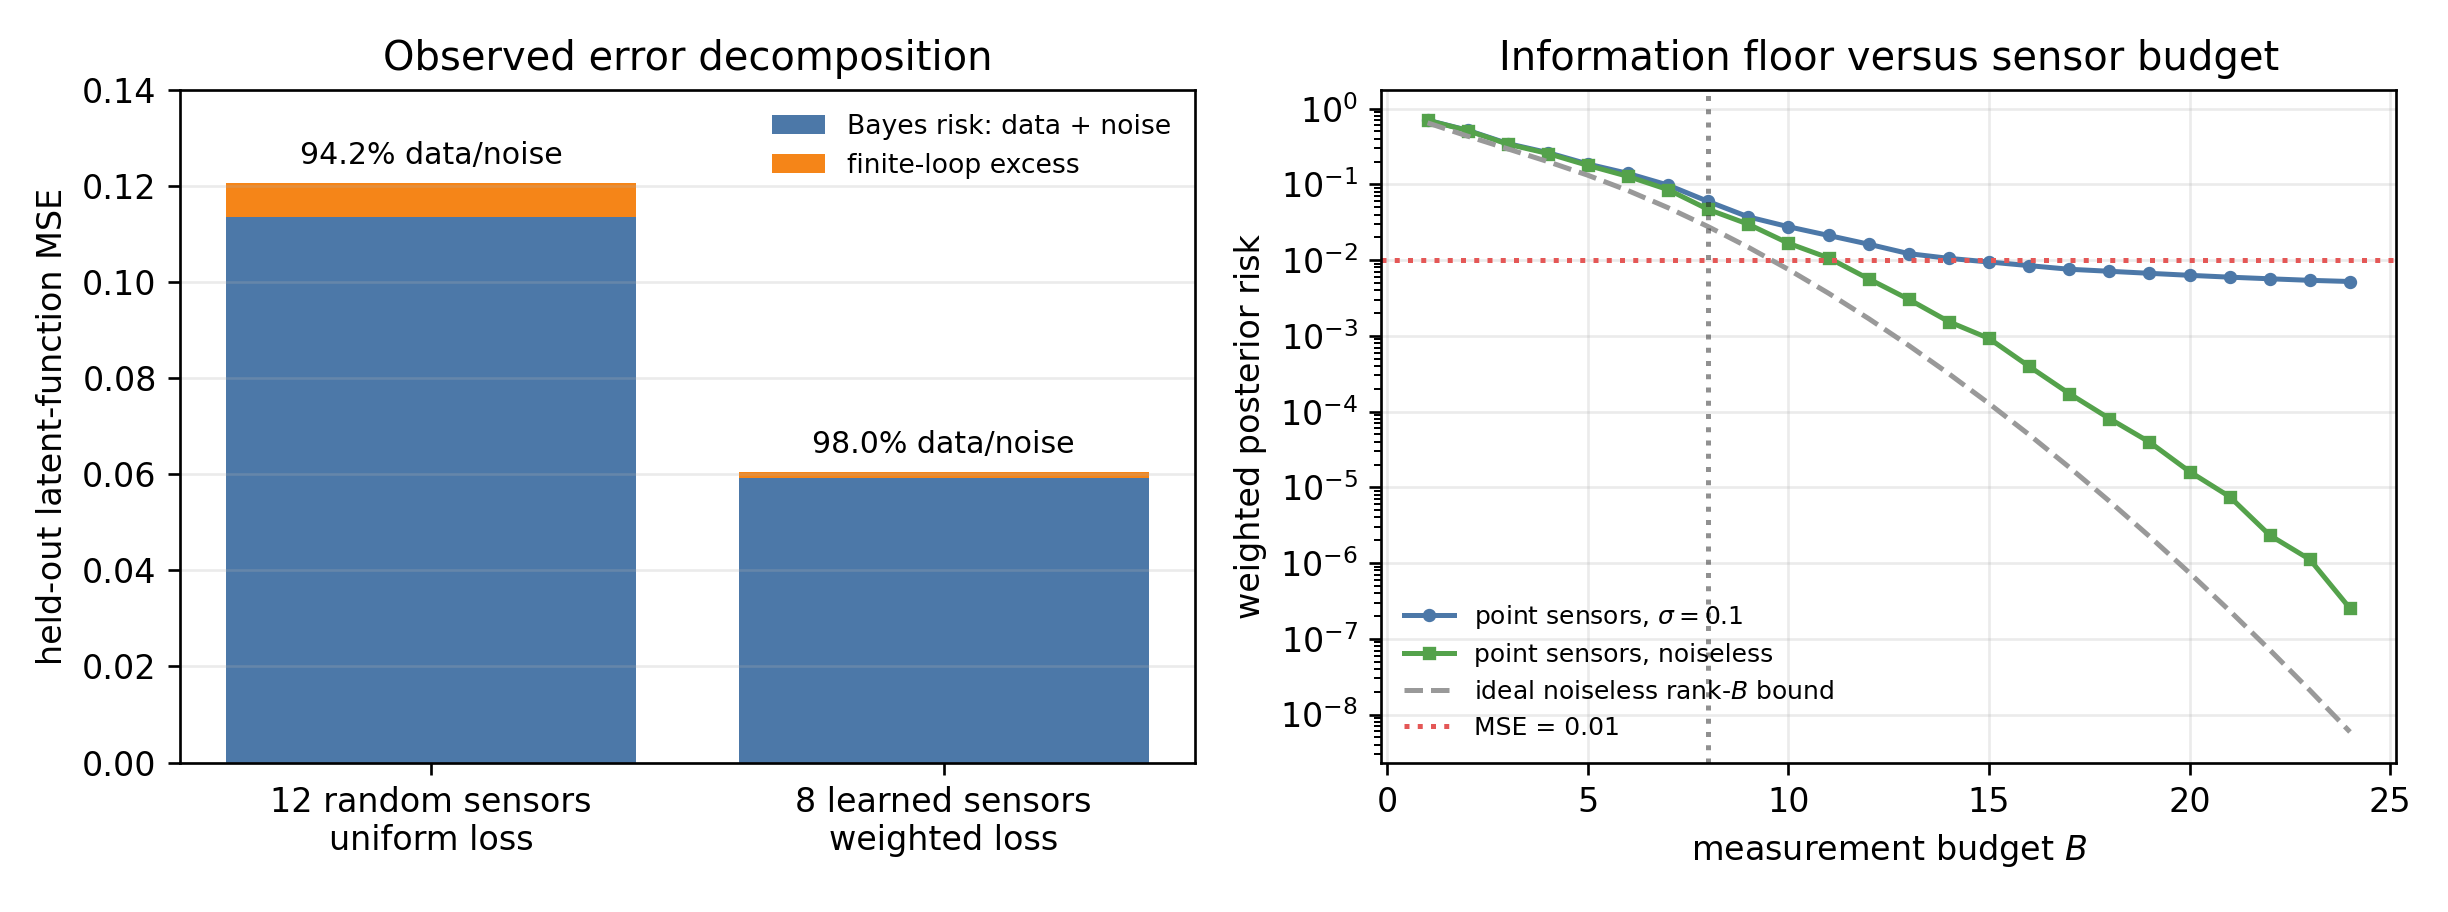
\includegraphics[width=\linewidth]{bottleneck_decomposition.png}
\caption{\textbf{Left:} almost all current error is the exact Bayesian risk
conditioned on the available measurements.  \textbf{Right:} analytic weighted
posterior risk for sequential point measurements, with and without observation
noise.  The grey curve is the more optimistic spectral lower bound obtained if
one were allowed arbitrary noiseless rank-$B$ linear measurements rather than
point sensors.  The current budget $B=8$ is marked vertically.}
\label{fig:bottleneck}
\end{figure}

\clearpage
\section{The primary bottleneck is the measurement budget}

At budget 8, three effects can be separated analytically for the weighted
design objective:
\begin{center}
\begin{tabular}{lc}
\toprule
Quantity & weighted posterior risk \\
\midrule
Ideal noiseless rank-8 linear-information bound & $0.02765$ \\
Greedy point design, noiseless & $0.04669$ \\
Greedy point design, $\sigma=0.1$ & $0.05950$ \\
Trained point design + exact GP, $\sigma=0.1$ & $0.05929$ \\
Trained point design + loop, $\sigma=0.1$ & $0.06049$ \\
\bottomrule
\end{tabular}
\end{center}
Even an unrealistically favourable noiseless linear sensing operator cannot
make the rank-8 risk much smaller than $2.8\times10^{-2}$ under this prior.
Restricting observations to locations raises the risk further, and noise adds
another $1.28\times10^{-2}$ for the greedy point design.  By contrast, the
finite loop contributes only $1.20\times10^{-3}$ for the trained design.

The regime changes near 16 well-placed sensors.  For the same weighted
objective, greedy posterior risks are
\begin{center}
\begin{tabular}{rcccccc}
\toprule
$B$ & 8 & 10 & 12 & 14 & 16 & 24 \\
\midrule
$\sigma=0.1$ & .05950 & .02760 & .01624 & .01056 & .00846 & .00522 \\
noiseless & .04669 & .01670 & .00566 & .00154 & .000395 & $<10^{-7}$ \\
\bottomrule
\end{tabular}
\end{center}
Thus $B\simeq16$ is the first sensible operating point for an MSE target below
$10^{-2}$.  Once the domain is adequately covered, observation noise becomes
the leading term; repeated measurements or lower-noise sensors then matter
more than additional training.

\section{The reported design loss was not a global reconstruction loss}

The design experiment minimized
\[
 \risk_w(\widehat f)
 =\sum_{q=1}^{64}w(x_q)\bigl(\widehat f(x_q)-f(x_q)\bigr)^2,
 \qquad
 w(x)\propto 0.2+\exp\!\left[-\frac{x^2}{2(0.32)^2}\right].
\]
Consequently $w(0)/w(\pm1)=5.78$.  Boundary errors are deliberately cheap.
This was useful for testing whether a policy could adapt to a nonuniform query
distribution, but it was the wrong objective for demonstrating visually good
reconstruction over the full interval.  The previous qualitative panel also
showed one arbitrary draw without uncertainty, which made the numerical result
hard to interpret.

Figure~\ref{fig:representative} uses a held-out episode selected as the median
exact-GP weighted error among 512 fresh draws, rather than selecting an easy
example.  With the current learned $B=8$ design, the global MSE is $0.145$ even
though the weighted MSE is $0.061$.  Running the same loop for 32 iterations
makes it coincide with the exact posterior mean but leaves the global MSE at
$0.140$.  Changing the information set to 16 globally placed measurements
reduces it to $0.010$.  The posterior band makes the missing information
visible and distinguishes uncertainty from solver error.

\begin{figure}[t]
\centering
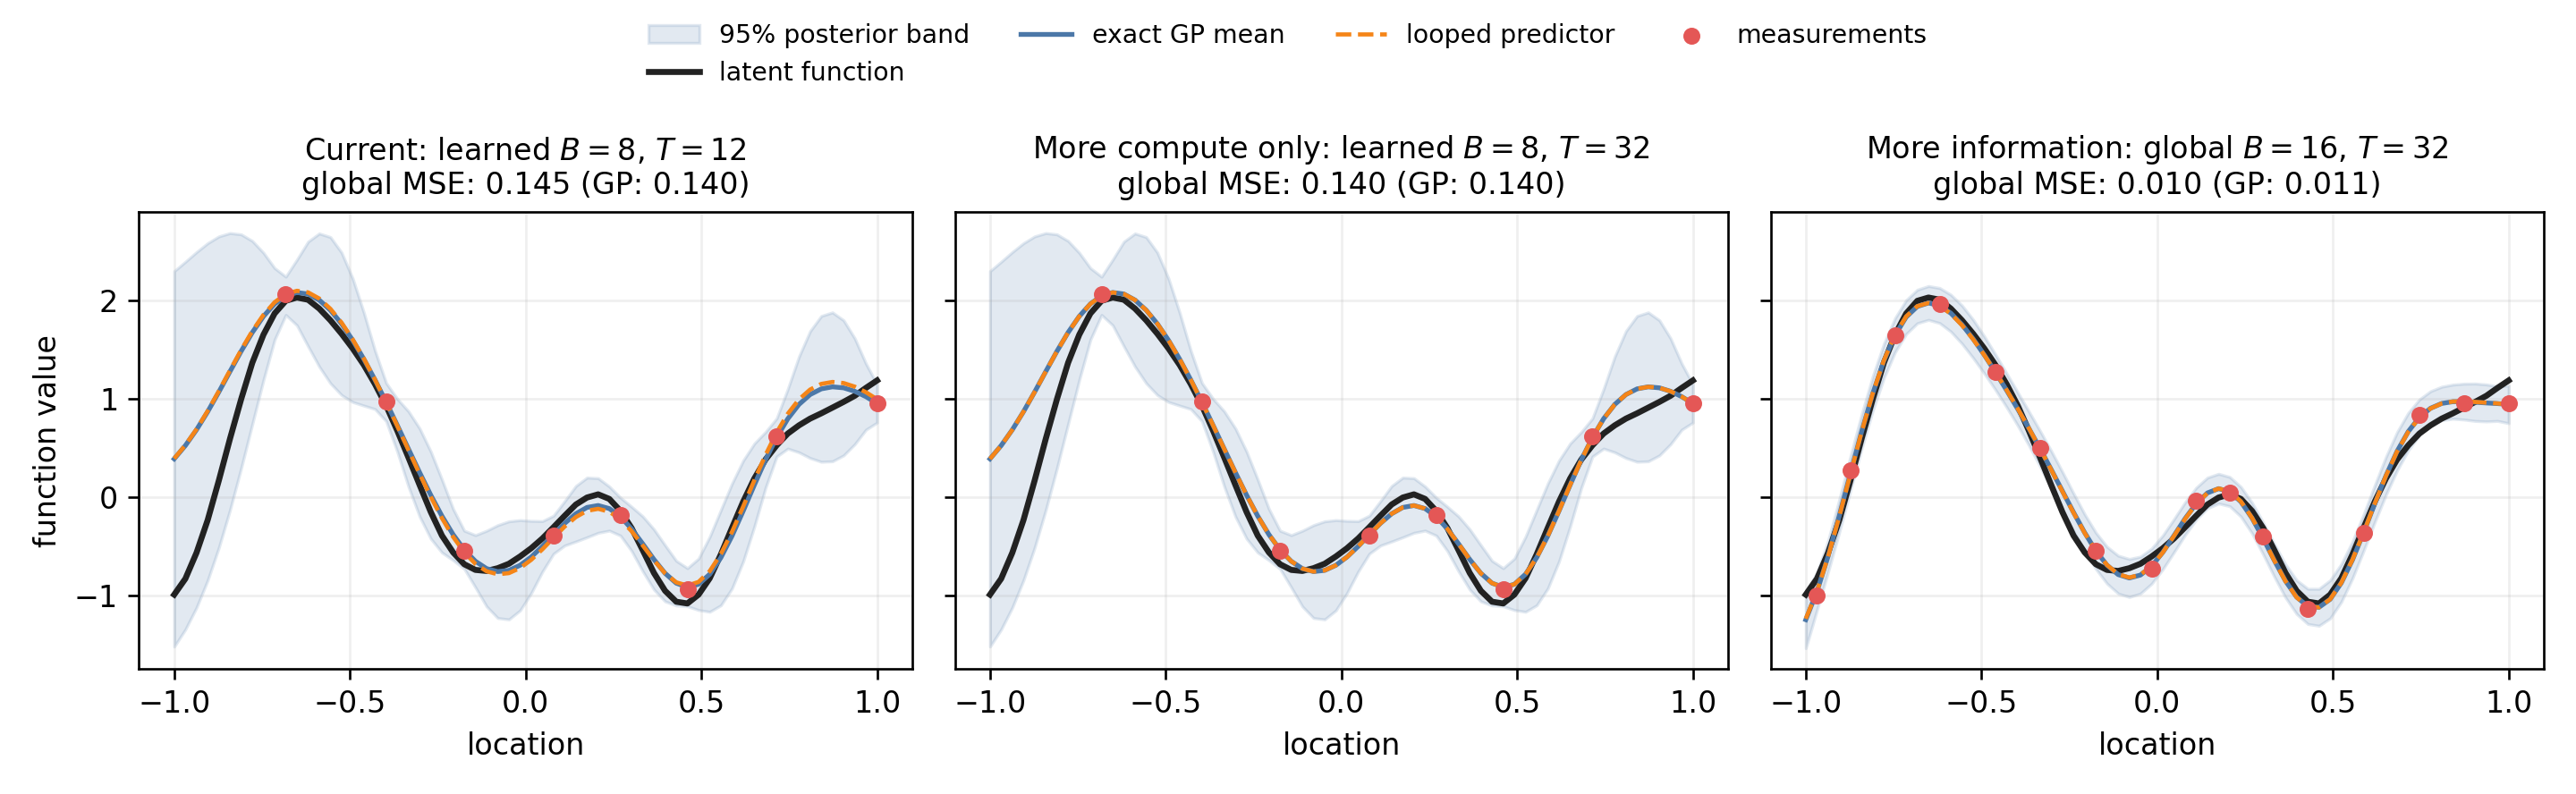
\includegraphics[width=\linewidth]{representative_reconstruction_en.png}
\caption{A representative held-out function.  More recurrent computation
aligns the loop with the exact GP mean but cannot recover the unobserved left
boundary.  Doubling the budget and optimizing global coverage removes the
dominant uncertainty and produces a genuinely accurate reconstruction.}
\label{fig:representative}
\end{figure}

\clearpage
\section{What should change in the next experiment}

If the target is small \emph{global} reconstruction error, the next protocol
should make the following changes.
\begin{enumerate}
  \item Replace the centre-weighted loss by uniform integrated MSE, or by a
  robust combination of integrated and worst-location posterior risk.
  \item Train and evaluate designs at budgets $B\in\{12,16,20,24\}$; retain
  $B=8$ only as a deliberately underdetermined stress test.
  \item Use 24--32 tied iterations at inference.  This removes nearly all of
  the solver excess without changing the fixed nonlinear feature geometry.
  \item Report exact-GP risk, loop excess, global MSE, weighted MSE, and
  posterior calibration separately.  A single loss number is insufficient.
  \item For the fixed LSM/PDE geometry, compute the same posterior trace before
  training.  This determines whether the proposed sensor budget can possibly
  attain the desired tolerance and prevents spending training time below an
  information-theoretic floor.
\end{enumerate}

The modelling conclusion about the nonlinearity remains intact: choosing the
softmax feature map to match the kernel is consequential.  At 12 observations,
the matched loop has MSE $0.1205$, compared with $0.2090$ for the same loop with
length scale $\ell/2$ and $0.1370$ for the standard Transformer.  What that
choice cannot do is manufacture information absent from the measurements.

\section{Scope}

These numbers concern a finite 64-point, one-dimensional RBF GP with fixed
geometry.  The spectral curve is a model-conditioned Bayesian bound, not a
universal scaling law, and the experiment is not yet evidence for a PDE
inverse problem.  Its useful conclusion is narrower and operational: the
present reconstruction plateau is caused chiefly by an undersized and
misaligned measurement objective, while the learned loop is already close to
the exact kernel regressor.

\end{document}
